\begin{XeClass}{FilterFileSystem}
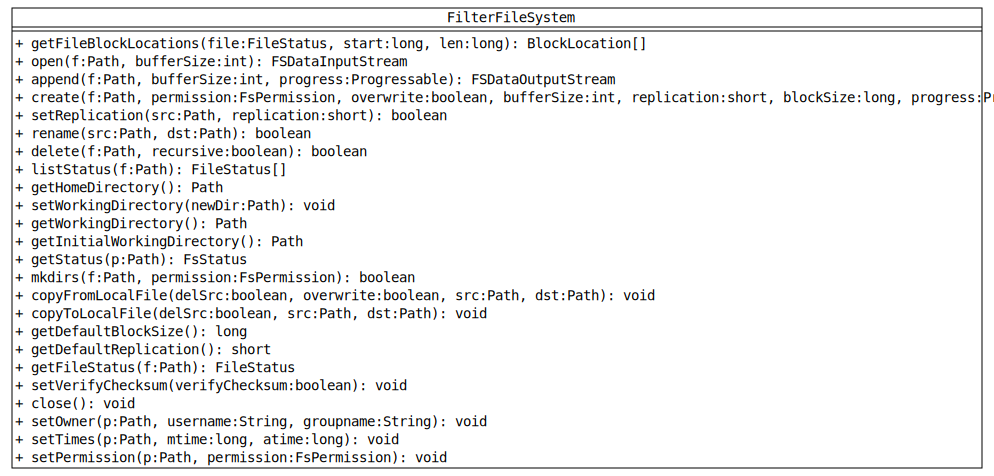
\includegraphics[width=\textwidth]{cdig/FilterFileSystem.png}
     
 FilterFileSystem继承了FileSystem类,重写了父类的所有方法 。
 FilterFileSystem是一个代理, 或者说, wrapper。
 类中包含一个FileSystem实例,用来作为基础的文件系统,在其中给
 它转换数据或者增加方法,加以封装,相当于起到了过滤文件系统的作用。
 Filter意为过滤器,FilterFileSystem选择的过滤策略是"直通",
 即什么都不做, 直接把参数传递给public方法对应的protected方法.
 FilterFileSystem包装了一个FileSystem对象,所有提供的方法都是与
 FileSystem中相同的方法,通过调用FileSystem对象对应的函数来实现,
 来为各方法添加更多地功能。

    \begin{XeMethod}{\XePublic}{BlockLocation[]}{getFileBlockLocations}
         
 获取文件的块位置信息

    \end{XeMethod}

    \begin{XeMethod}{\XePublic}{FSDataInputStream}{open}
         
 打开一个文件数据的输出流

    \end{XeMethod}

    \begin{XeMethod}{\XePublic}{FSDataOutputStream}{append}
         
 进行输出流的追加操作

    \end{XeMethod}

    \begin{XeMethod}{\XePublic}{FSDataOutputStream}{create}
         
 创建一个文件输出流
 the file will be overwritten, and if false an error will be thrown.

    \end{XeMethod}

    \begin{XeMethod}{\XePublic}{boolean}{setReplication}
         
 复制一个存在的文件
 false if file does not exist or is a directory

    \end{XeMethod}

    \begin{XeMethod}{\XePublic}{boolean}{rename}
         
 重命名文件,文件可以是本地文件系统和远程分布式文件系统

    \end{XeMethod}

    \begin{XeMethod}{\XePublic}{boolean}{delete}
         
 删除文件,可选择是否递归删除

    \end{XeMethod}

    \begin{XeMethod}{\XePublic}{FileStatus[]}{listStatus}
         
 列出文件状态

    \end{XeMethod}

    \begin{XeMethod}{\XePublic}{Path}{getHomeDirectory}
         
 获取home目录

    \end{XeMethod}

    \begin{XeMethod}{\XePublic}{void}{setWorkingDirectory}
         
 设置工作目录

    \end{XeMethod}

    \begin{XeMethod}{\XePublic}{Path}{getWorkingDirectory}
         
 获取工作目录

    \end{XeMethod}

    \begin{XeMethod}{\XeProtected}{Path}{getInitialWorkingDirectory}
         
 获取初始工作目录

    \end{XeMethod}

    \begin{XeMethod}{\XePublic}{FsStatus}{getStatus}
         
 获取文件状态

    \end{XeMethod}

    \begin{XeMethod}{\XePublic}{boolean}{mkdirs}
         
 根据路径和权限创建目录

    \end{XeMethod}

    \begin{XeMethod}{\XePublic}{void}{copyFromLocalFile}
         
 从本地文件系统复制

    \end{XeMethod}

    \begin{XeMethod}{\XePublic}{void}{copyToLocalFile}
         
 复制到本地文件系统

    \end{XeMethod}

    \begin{XeMethod}{\XePublic}{long}{getDefaultBlockSize}
         
 获取默认块大小

    \end{XeMethod}

    \begin{XeMethod}{\XePublic}{short}{getDefaultReplication}
         
 获得默认副本

    \end{XeMethod}

    \begin{XeMethod}{\XePublic}{FileStatus}{getFileStatus}
         
 Get file status.
 获取文件状态信息

    \end{XeMethod}

    \begin{XeMethod}{\XePublic}{void}{setVerifyChecksum}
         
 设置确认校验和的布尔变量

    \end{XeMethod}

    \begin{XeMethod}{\XePublic}{void}{close}
         
 关闭文件系统实例

    \end{XeMethod}

    \begin{XeMethod}{\XePublic}{void}{setOwner}
         
 设置文件拥有者

    \end{XeMethod}

    \begin{XeMethod}{\XePublic}{void}{setTimes}
         
 设置时间,包括修改时间和访问时间

    \end{XeMethod}

    \begin{XeMethod}{\XePublic}{void}{setPermission}
         
 设置文件权限

    \end{XeMethod}

\end{XeClass}
